\documentclass[a4paper]{article}
\usepackage[UTF8]{ctex}
\usepackage{geometry}
\usepackage{graphicx}
\usepackage{url}
\usepackage{multirow}
\usepackage{array}
\usepackage{booktabs}
\usepackage{url}
\usepackage{enumitem}
\usepackage{graphicx}
\usepackage{float}
\usepackage{amssymb}
\usepackage{amsmath}
\usepackage{subfig}
\usepackage{longtable}
\usepackage{pifont}
\usepackage{color}

\allowdisplaybreaks

\geometry{a4paper, scale=0.78}

% \begin{figure}[H]
%     \centering
%     \includegraphics[width=.55\textwidth]{E.png}
%     \caption{矩阵与列向量的乘法}
%     \label{fig:my_label_1}
% \end{figure}


% \left\{
% \begin{array}{ll}
%       x+2x+z=2 & \\
%       3x+8y+z=12 & \\
%       4y+z=2
% \end{array}
% \right.

% \begin{enumerate}[itemindent = 1em, itemsep = 0.4pt, parsep=0.5pt, topsep = 0.5pt]

% \end{enumerate}

%\stackrel{a}{\longrightarrow}

\title{Probability Graph 07 Variable Elimination}
\author{Chen Gong}
\date{07 December 2019}
\begin{document}
\maketitle
在上一小节中,我们简单的介绍了推断的背景和分类,我们知道了大致有哪些推断的方法。推断的任务可以被我们介绍为:给定已知的$p(x) = (x_1,x_2,\cdots,x_p)$,我们需要求的有三个:

1. 边缘概率:$p(x_i) = \sum_{x_1,\cdots,x_{i-1},x_{i+1},\cdots,x_p}p(x_1,x_2,\cdots,x_p)$。

2. 条件概率:$p(x_A|x_B)$,也就是在已知$x_B$集合的情况下,如何求得$x_A$集合的概率。

3. 最大后验概率(MAP):$\hat{x}_A=\arg\max_{x_A}p(x_A|x_B) = \arg\max_{x_A}\ p(x_A,x_B)$。

下面我们要介绍最简单的一个精确推断中中的东西,名为变量消除法(Variable Elimination)。这是一种最简单的推断方法,也是我们学习推断法的核心概念之一。下面我们做详细的解释。

\section{变量消除法(Variable Elimination Algorithm)}
假如我们有一个马氏链:
\begin{figure}[H]
    \centering
    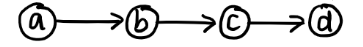
\includegraphics[width=.45\textwidth]{微信图片_20191207173240.png}
    \caption{一个马氏链的抽象模型}
    \label{fig:my_label_1}
\end{figure}

那么我们怎么来求$p(d)$呢?根据公式我们可以得到:
\begin{equation}
    p(d) = \sum_{a,b,c}p(a,b,c,d)
\end{equation}

然后使用因子分解,我们可以得到:
\begin{equation}
    p(d) = \sum_{a,b,c}p(a)p(b|a)p(c|b)p(d|c)
\end{equation}

假定,$a,b,c,d$都为均匀离散的二值random variable,所以$a,b,c,d\in \{0,1\}$。

所以,
\begin{equation}
    \begin{split}
        p(d) = & p(a=0)\cdot p(b=0|a=0) \cdot p(c=0|b=0) \cdot p(d|c=0) \\
        + & p(a=1)\cdot p(b=0|a=1) \cdot p(c=0|b=0) \cdot p(d|c=0) \\
        + & \cdots \\
        + & p(a=1)\cdot p(b=1|a=1) \cdot p(c=1|b=1) \cdot p(d|c=1) \\
    \end{split}
\end{equation}
实际上,这里有8个因子的积。那么我们来做进一步的分析,我们可以令
\begin{equation}
    \begin{split}
        p(d) 
        = & \sum_{a,b,c}p(a)p(b|a)p(c|b)p(d|c) \\
        = & \sum_{b,c}p(c|b)p(d|c)\sum_a p(a)p(b|a)
    \end{split}
\end{equation}

而$p(a)p(b|a) = p(a,b)$,而$\sum_a p(a)p(b|a) = p(b)$。我们可以将$a$看成$\phi(a)$这是一个和$a$相关的函数,同理$p(b|a)$看成$\phi(a,b)$。所以,我们可以将$\sum_a p(a)p(b|a)$看成$\phi_a(b)$,这样就相当于一个关于$b$的函数,并且是从$a$中导出的。所以,我们做如下替换可得:
\begin{equation}
    \sum_{b,c}p(c|b)p(d|c)\sum_a p(a)p(b|a) = \sum_{b,c}p(c|b)p(d|c)\phi_a(b)=\sum_c p(d|c)\sum_b p(c|b)\phi_a(b)
\end{equation}

同理,我们将$\sum_b p(c|b)\phi_a(b)$看成$\phi_b(c)$。所以,原始将被改写为:
\begin{equation}
    \sum_cp(d|c)\phi_b(c) = \phi_c(d)
\end{equation}

这个算法的核心就是乘法对加法的分配律。那我们怎么类比到乘法的分配律呢?首先先来简单的回顾一下乘法的分配律,也就是$ac+ab=a(b+c)$。那么我们仔细的来看看这个计算$p(d)$的过程。这是不是就是一个不断的提取公因子,进行计算的过程?有没有觉得和分配律很像?先提取$a$的部分,计算$a$的部分,然后再依次的提取$b$的部分,$c$的部分,最后剩下的就是$d$的部分。那么,我们就可以把这么一长串的公式进行逐步化简了,这就是变量消元的思想。同样,在无向图中,我们也可以使用到马尔可夫网络中。
\begin{equation}
    p(a,b,c,d) = \frac{1}{z}\prod_{i=1}^k \phi_{c_i}(x_{c_i})
\end{equation}
写成因子分解的形式就是$p(x) = \prod_{x_i}\phi_i(x_i)$。这实际上就是分配律,一个变量一个变量的提取,然后进行分解计算。同时这种算法的缺点也非常的明显。

首先,就是重复计算的问题,无论计算那个变量的概率都要重复的计算一遍所有的概率。这个原因就会导致算法的计算难度非常的大。第二个就是计算次序的问题,我们举的例子还比较的简单,所以我们可以一眼就看出来,按$a-b-c-d$的次序开始算。但是,实际上,并没有这么容易就得到计算的次序,而且计算次序不一样会导致计算的难度有很大的区别。而有数学家已经证明了,确定最优的计算顺序,本身就是一个NP hard的问题,非常难求解。
























\end{document}
